\documentclass[12pt, a4paper]{article}
\usepackage[utf8]{inputenc}
\usepackage{amsmath}
\usepackage{amsfonts}
\usepackage{amssymb}
\usepackage{graphicx}
\usepackage{caption}
\usepackage{subcaption}
\usepackage{sidecap}
\author{MORAES, FELIPE}
\title{Fundamentals of STDP based recurrent assembly networks}

\newtheorem{theorem}{Theorem}[section]
\newtheorem{lemma}[theorem]{Lemma}
\newtheorem{proposition}[theorem]{Proposition}
\newtheorem{corollary}[theorem]{Corollary}

\newenvironment{proof}[1][Proof]{\begin{trivlist}
\item[\hskip \labelsep {\bfseries #1}]}{\end{trivlist}}
\newenvironment{definition}[1][Definition]{\begin{trivlist}
\item[\hskip \labelsep {\bfseries #1}]}{\end{trivlist}}
\newenvironment{example}[1][Example]{\begin{trivlist}
\item[\hskip \labelsep {\bfseries #1}]}{\end{trivlist}}
\newenvironment{remark}[1][Remark]{\begin{trivlist}
\item[\hskip \labelsep {\bfseries #1}]}{\end{trivlist}}

\newcommand{\qed}{\nobreak \ifvmode \relax \else
      \ifdim\lastskip<1.5em \hskip-\lastskip
      \hskip1.5em plus0em minus0.5em \fi \nobreak
      \vrule height0.75em width0.5em depth0.25em\fi}

\renewcommand{\figurename}{Figura}

\begin{document}

\begin{center}
{\huge TRABALHO PRÁTICO 1: Emulador}
\textit{Felipe Moraes Gomes - felipemoraes@dcc.ufmg.br}
\end{center}
\section{Introdução e Definição do Trabalho}
Este trabalho descreve a implementação e operação de um simulador para um processador hipotético baseado na arquitetura RISC. A máquina virtual recebe como entrada um binário, e alguns parâmetros de execução, que ele então usa para interpretar o código lido.

O restante deste documento está organizado da seguinte forma: A 2\textsuperscript{a} seção trata da implementação da máquina virtual e sua organização no código; A 3\textsuperscript{a} seção explicita o formato de execução, entrada e saída do programa; A 4\textsuperscript{a} seção contém os testes realizados; A 5\textsuperscript{a} seção contém algumas considerações finais, concluindo o trabalho. Após isso, é colocado um apêndice contendo uma listagem dos arquivos do projeto. 

\section{Implementação e Organização}

A máquina virtual carrega as instruções do arquivo de entrada especificado e as executa uma a uma até a conclusão do programa. A máquina virtual é implementada por meio de duas funções \emph{Load} e \emph{Execute}, delineada a seguir.

\subsection{Dados e Variáveis}

O algoritmo principal define várias estruturas de dados, todas de acesso global. Algumas das declarações são do tipo \emph{int}, que é um inteiro de 32 bits.

\begin{itemize}
\item \emph{int Mem[1000]}: A memória principal da máquina.
\item \emph{int PC, SP}: Os registradores de uso específico; O PC (Program Counter) mantém o índice da instrução sendo executada; O SP (Stack Pointer) aponta para o topo da pilha. 
\item \emph{int R[8]}: Os 8 registradores de uso geral; Os nomes de cada registrador estão associados a seus respectivos índices pelo pseudônimos \emph{RA} = 0, \emph{RB} = 1, \emph{RC} = 2 e \emph{RD} = 3;
\item \emph{char PSW[2]}: Os flags setados durante as operações de \emph{COPY} e \emph{ALU}, e usados pelas funções de branch; O primeiro (\emph{PSW[0] - Zero Flag}) é setado quando o resultado destas operações for 0, e o segundo (\emph{PSW[1] - Sign Flag}) quando o bit de sinal (o mais significativo) for 1.
\end{itemize}

\subsection{Métodos e Funções}

\begin{itemize}
\item \emph{int Load()}: Confere o arquivo binário e em seguida carrega o programa na memória. 
\item \emph{int Execute(int code)}: Lê a instrução corrente e seus operandos da memória de acordo com o PC e a executa, retornando o status da execução daquela instrução. As instruções são decodificadas por um \emph{switch}, que efetua as operações do conjunto de instruções, caso o status retornado identifique uma instrução halt, o emulador é finalizado. Quando uma instrução desconhecida é lida, a função não executa nenhuma instrução e incrementa o PC em um para o programa continuar a sua execução na próxima instrução.
\end{itemize}

\subsection{Fluxo de Execução}

O programa inicialmente lê os parametros passados a ele, verificando sua validade. Caso o formato esteja correto ele carrega o programa chamando \emph{Load}. Havendo êxito, \emph{Execute} é chamado. Ao retornar, o programa conclui sua execução caso status identifique uma instrução halt.

\section{Controle \& IO}

\subsection{Execução e Compilação do Emulador}

O programa pode ser compilado através do gcc, pelo utilitário \emph{make}, usando o makefile providenciado. Uma vez compilado, chamadas devem seguir o formato:

\begin{center}
\emph{./emulador input.mk `s'{\tt{|}}`v'}
\end{center}

Onde `s' especifica que a saída deve ser simples (somente com os resultados de execuções de \emph{WRITE} e \emph{READ}), enquanto `v' especifica que o programa deve também imprimir o banco de registradores, flags e instrução corrente a cada passo. \emph{input} é o nome do arquivo que contém o código binário a ser interpretado.

\subsection{Formato dos Binários}

Os programas executados pela máquina virtual são codificados em arquivos binários, onde os dois primeiros bytes contém a assinatura do binário ("M" e "K"), os próximos 4 bytes o PC e em seguida 4 bytes que corresponde ao valor do s próximos bytes correspondem exatamente a um \emph{int}, que representa um dado ou uma instrução, segundo a codificação apresentada na especificação.

\subsection{Interação em Tempo de Execução}

São definidas duas instruções que permitem interagir com os programas em tempo de execução, que são \emph{READ} e \emph{WRITE}, que usam a saida padrão (terminal) para se comunicarem com o usuário.

Execuções de \emph{READ} requisitam a entrada de um número na parte do usuário; Execuções de \emph{WRITE} imprime o valor corrente do endereço de memória especificado na instrução. 

\section{Testes}

\begin{figure}
\centering
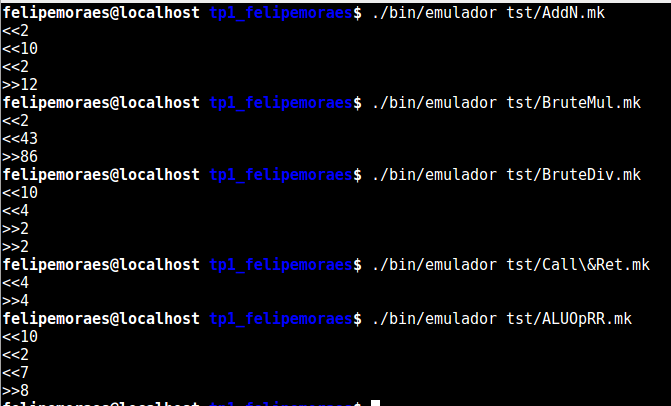
\includegraphics[width=1.1\textwidth]{RuntimeScreencap.png}
\caption{Execução dos testes}
\label{FigureExecution}
\end{figure}

Múltiplos testes foram efetuados sobre o emulador, de forma a obter cobertura total do código e do conjunto de instruções. Os testes foram executados com \emph{PC= 0} e \emph{SP = 1000}. As execuções de cada programa são ilustradas na Fig. \ref{FigureExecution}.

\begin{itemize}
\item \emph{Soma N (AddN.mk):} Calcula e imprime a soma de \emph{N} números, onde \emph{N} é o primeiro parâmetro, que vem seguido pelos \emph{N} números a serem somados.
\item \emph{Divisão força bruta (BruteDiv.mk):} Faz a divisão força bruta de dois números (passados como parâmetros), e imprime o quociente e o resto obtido.
\item \emph{Multiplicação força bruta (BruteMul.mk):} Faz a multiplicação força bruta de dois números (passados como parâmetros), e imprime o produto obtido.
%\item \emph{Fibonacci (Fibonacci.sbexe)}: Imprime o enésimo número da sequência fibonacci, onde \emph{N} é passado como parâmetro.
%\item \emph{Mediana de 7 (Median7.sbexe)}: Dado um conjunto de 7 números (lidos do terminal), imprime sua mediana.
\item \emph{Cobertura (ALUOpRR.mk)}: Testa as instruções não abordadas pelos programas anteriores; O teste lê dois parâmetros \emph{A}, \emph{B} e \emph{C}, e imprime um valor de acordo com o parâmetro \emph{C} o tipo de operação lógica e aritmética de acordo com o código da instrução de operações Registrador-Registradore. 
\item \emph{Cobertura (Call{\&}Ret.mk)}: Testa a máquina virtual para chamadas de funções e retorno de parâmetros. Recebe um parâmetro \emph{A} e retorna o mesmo valor caso todas chamadas foram bem sucedidas.
\end{itemize}

\section{Conclusão}

O emulador é um interpretador eficiente e eficaz da linguagem especificada, oferecendo reconhecimento de instruções comparáveis com aquelas fornecidas pelo RISC. 

O baixo número de registradores e a falta de endereçamento imediato, no entanto, tornam a arquitetura desta máquina incompatível com problemas de maior escala, que teria de recorrer à memória com uma alta frequência, acarretando em delays intoleráveis para muitas aplicações de uso comum.

Evidentemente, conceitos mais avançados associados a essa arquitetura (como pipeline) foram omitidas pelo fato das mesmas não contribuírem para o melhor reconhecimento da linguagem.

A execução do trabalho transcorreu sem maiores dificuldades, e os resultados obtidos correspondem ao esperado.

\appendix
\section{Apêndice}
\subsection{Listagem de Arquivos}
\begin{itemize}
	\item Código Fonte:
	\begin{itemize}
		\item \emph{src/main.c:} Interpreta os parâmetros de entrada e controla o fluxo do programa (Seção 2.1).
		\item \emph{src/func.c, src/func.h:} Implementa a máquina virtual (Seção 2.2).
	\end{itemize}
	\item Testes:
	\begin{itemize}
		\item \emph{tst/AddN.mk:} (Seção 4 item 1).
		\item \emph{tst/BruteDiv.mk:} (Seção 4 item 2).
		\item \emph{tst/BruteMul.mk:} (Seção 4 item 3).
		\item \emph{tst/ALUOpRR.mk:} (Seção 4 item 4).
		\item \emph{tst/Call{\&}Ret.mk:} (Seção 4 item 3).
%		\item \emph{tst/Fibonacci.sbexe:} (Seção 4 item 4).
%		\item \emph{tst/Median7.sbexe:} (Seção 4 item 5).
%		\item \emph{tst/Logic{\&}BNZ.sbexe:} (Seção 4 item 6).
	\end{itemize}
	
\end{itemize}

\end{document}
